\documentclass{beamer}
\usetheme{Warsaw}

\usepackage[utf8]{inputenc}
\usepackage{fancybox}
\usepackage{multimedia} 
\usepackage{subfig}
\usepackage{amsmath}
\usepackage{hyperref}
\hypersetup{
    colorlinks=true,     
    urlcolor=blue
}
\usepackage[all]{xy}

\setbeamertemplate{footline}[frame number]


\begin{document}


\title[Stochastik] % (optional, only for long titles)
{Wahrscheinlichkeitstheorie und Statistik (Stochastik)
\\
\includegraphics[scale=0.5]{img/craps}
}
\subtitle{}
\author[Dr. Johannes Riesterer] % (optional, for multiple authors)
{Dr.  rer. nat. Johannes Riesterer}

\date[KPT 2004] % (optional)
{}

\subject{Stochastik}

\frame{\titlepage}

\begin{frame}
    \frametitle{Einleitung}
\framesubtitle{Was ist Stochastik?}
    \begin{block}{Wahrscheinlichkeitstheorie}
 Beschreibung und Untersuchung von zufälligen Vorgängen und Modellen.
\end{block}
    \begin{block}{Statistik}
Umgang mit dem Zufall und Schlussfolgern aus Beobachtungen
\end{block}
 \end{frame}

\begin{frame}
    \frametitle{Einleitung}
\framesubtitle{}


\begin{figure}[htp]
      \centering
    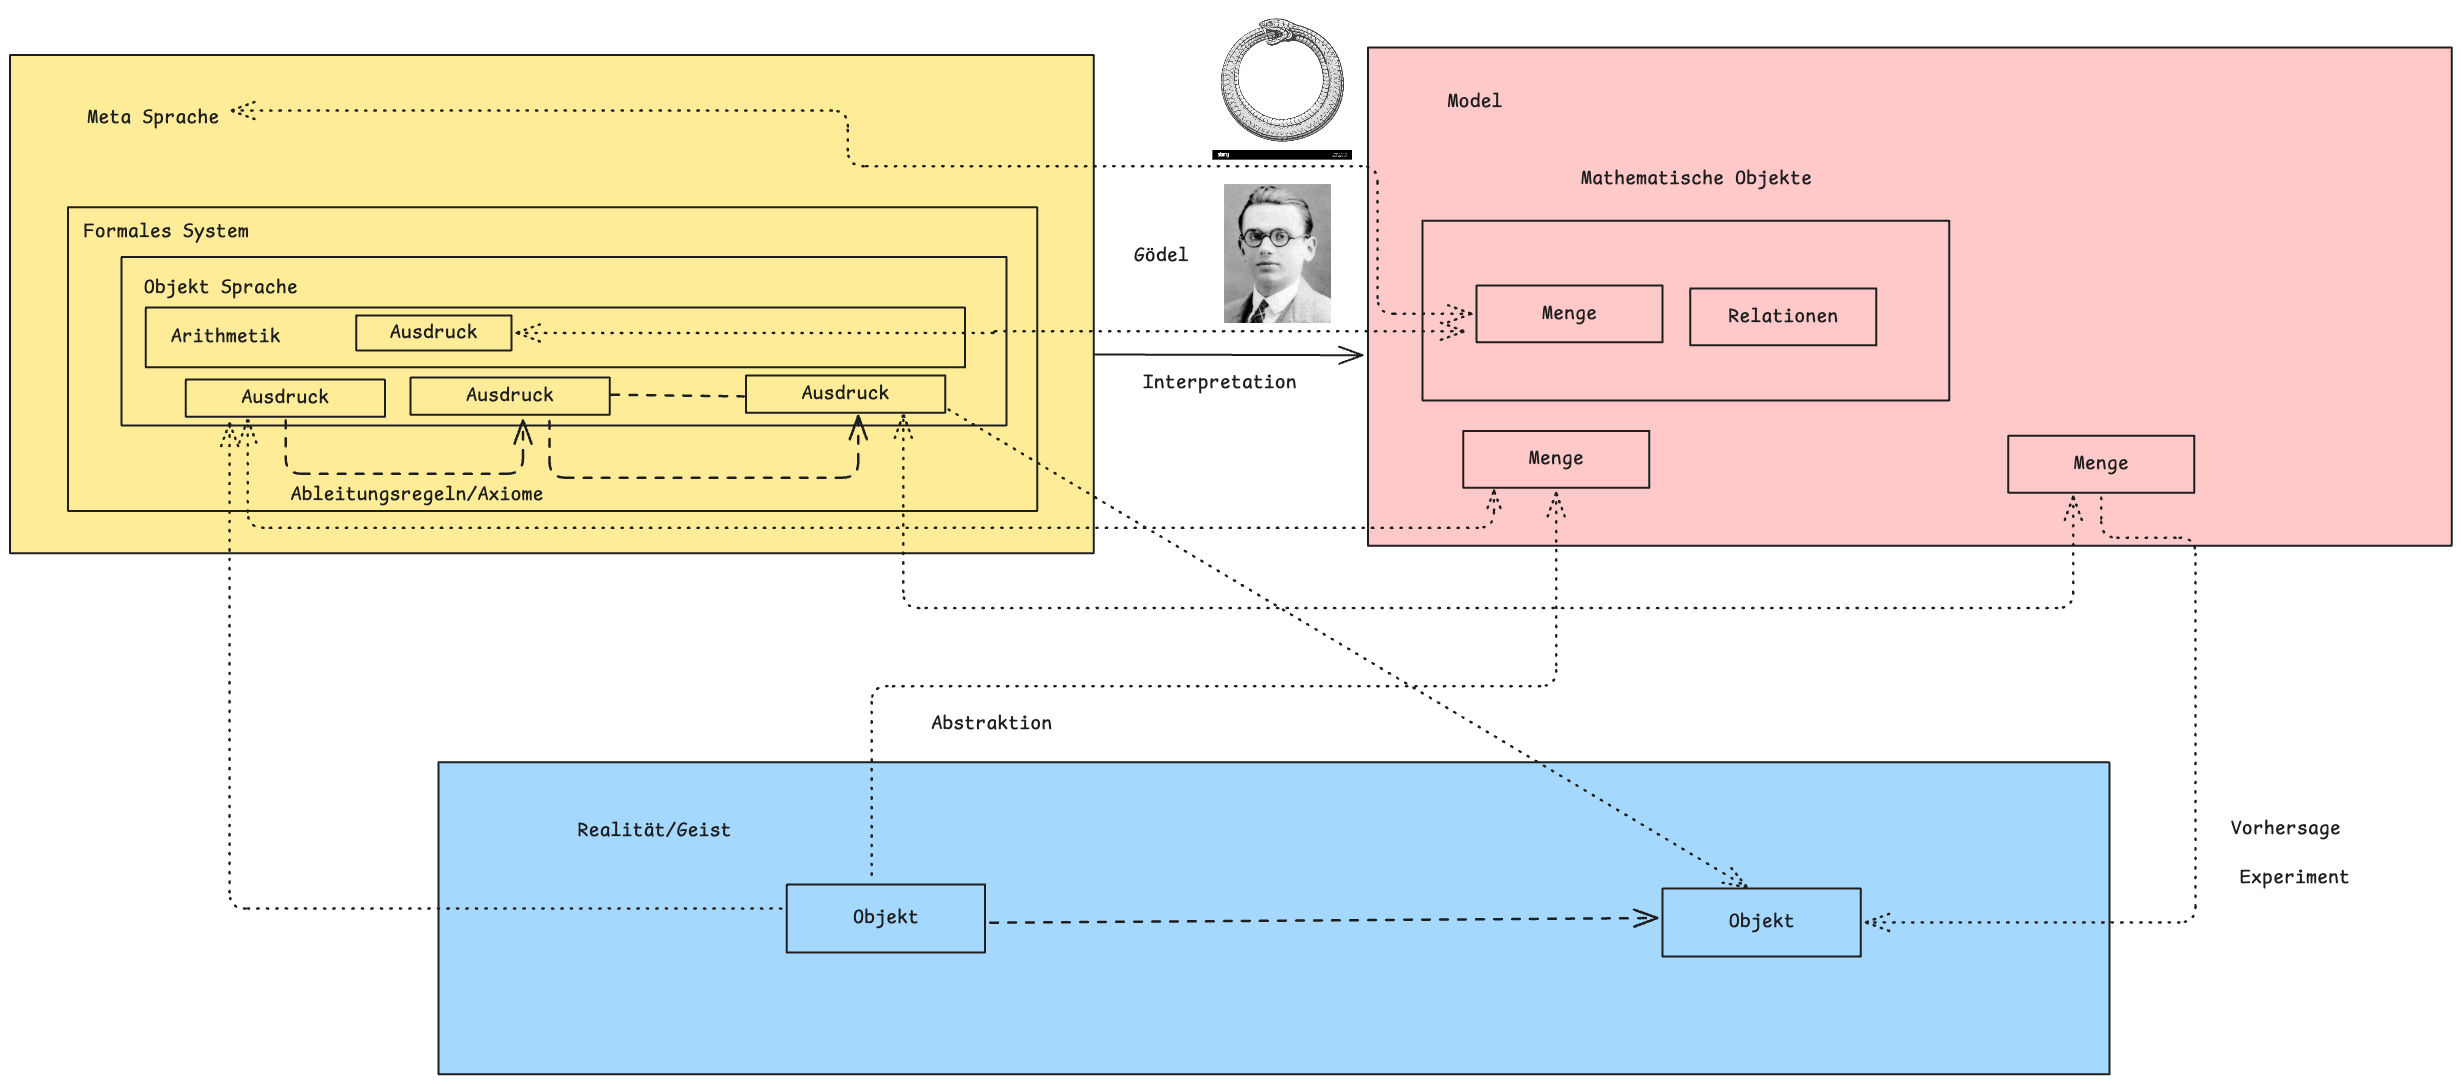
\includegraphics[width=1.0 \textwidth]{img/reality_vs_math.png}


\end{figure}
 \end{frame}


\begin{frame}
    \frametitle{Einleitung}
\framesubtitle{}

    \begin{block}{Was ist Zufall}
Keine kausale Erklärung für den Ausgang eines Vorganges vorhanden (Nicht-Deterministisch)
\end{block}



   \begin{block}{Kausalität (Wikipedia)}
Kausalität ist die Beziehung zwischen Ursache und Wirkung. Sie betrifft die Abfolge von Ereignissen und Zuständen, die aufeinander bezogen sind. Demnach ist A die Ursache für die Wirkung B, wenn B von A herbeigeführt wird.
\end{block}

\begin{figure}[htp]
      \centering
    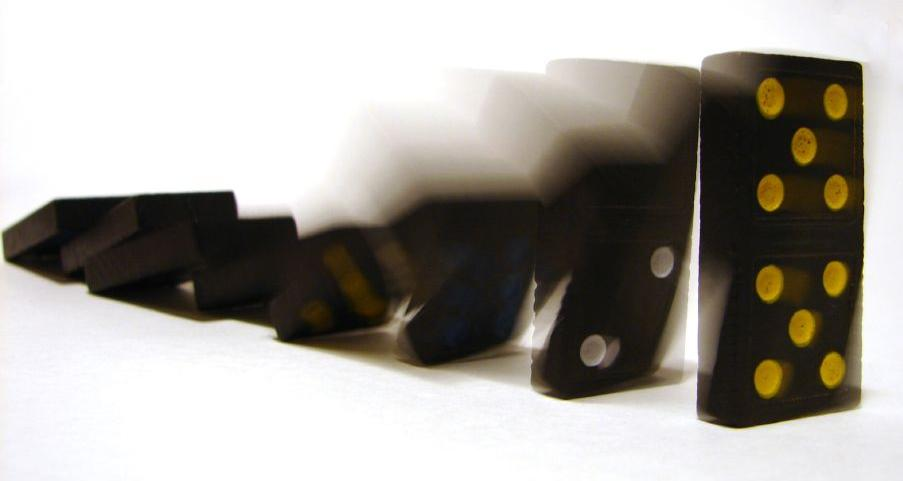
\includegraphics[width=0.3\textwidth]{img/Domino}

      \caption{Quelle: Wikipedia}
\end{figure}


\end{frame}



\begin{frame}
    \frametitle{Einleitung}
\framesubtitle{}

    \begin{block}{Stochastik vs. Kausalität}
Beobachtung: Bei Regen tragen die Menschen einen Regenschirm.
Es folgt NICHT: Wenn man einen Regenschirm aufspannt, fängt es an zu regnen.
Ebenso folgt NICHT: Wenn es regnet, sieht man Menschen mit Regenschirmen. 
\end{block}


\begin{figure}[htp]
      \centering
    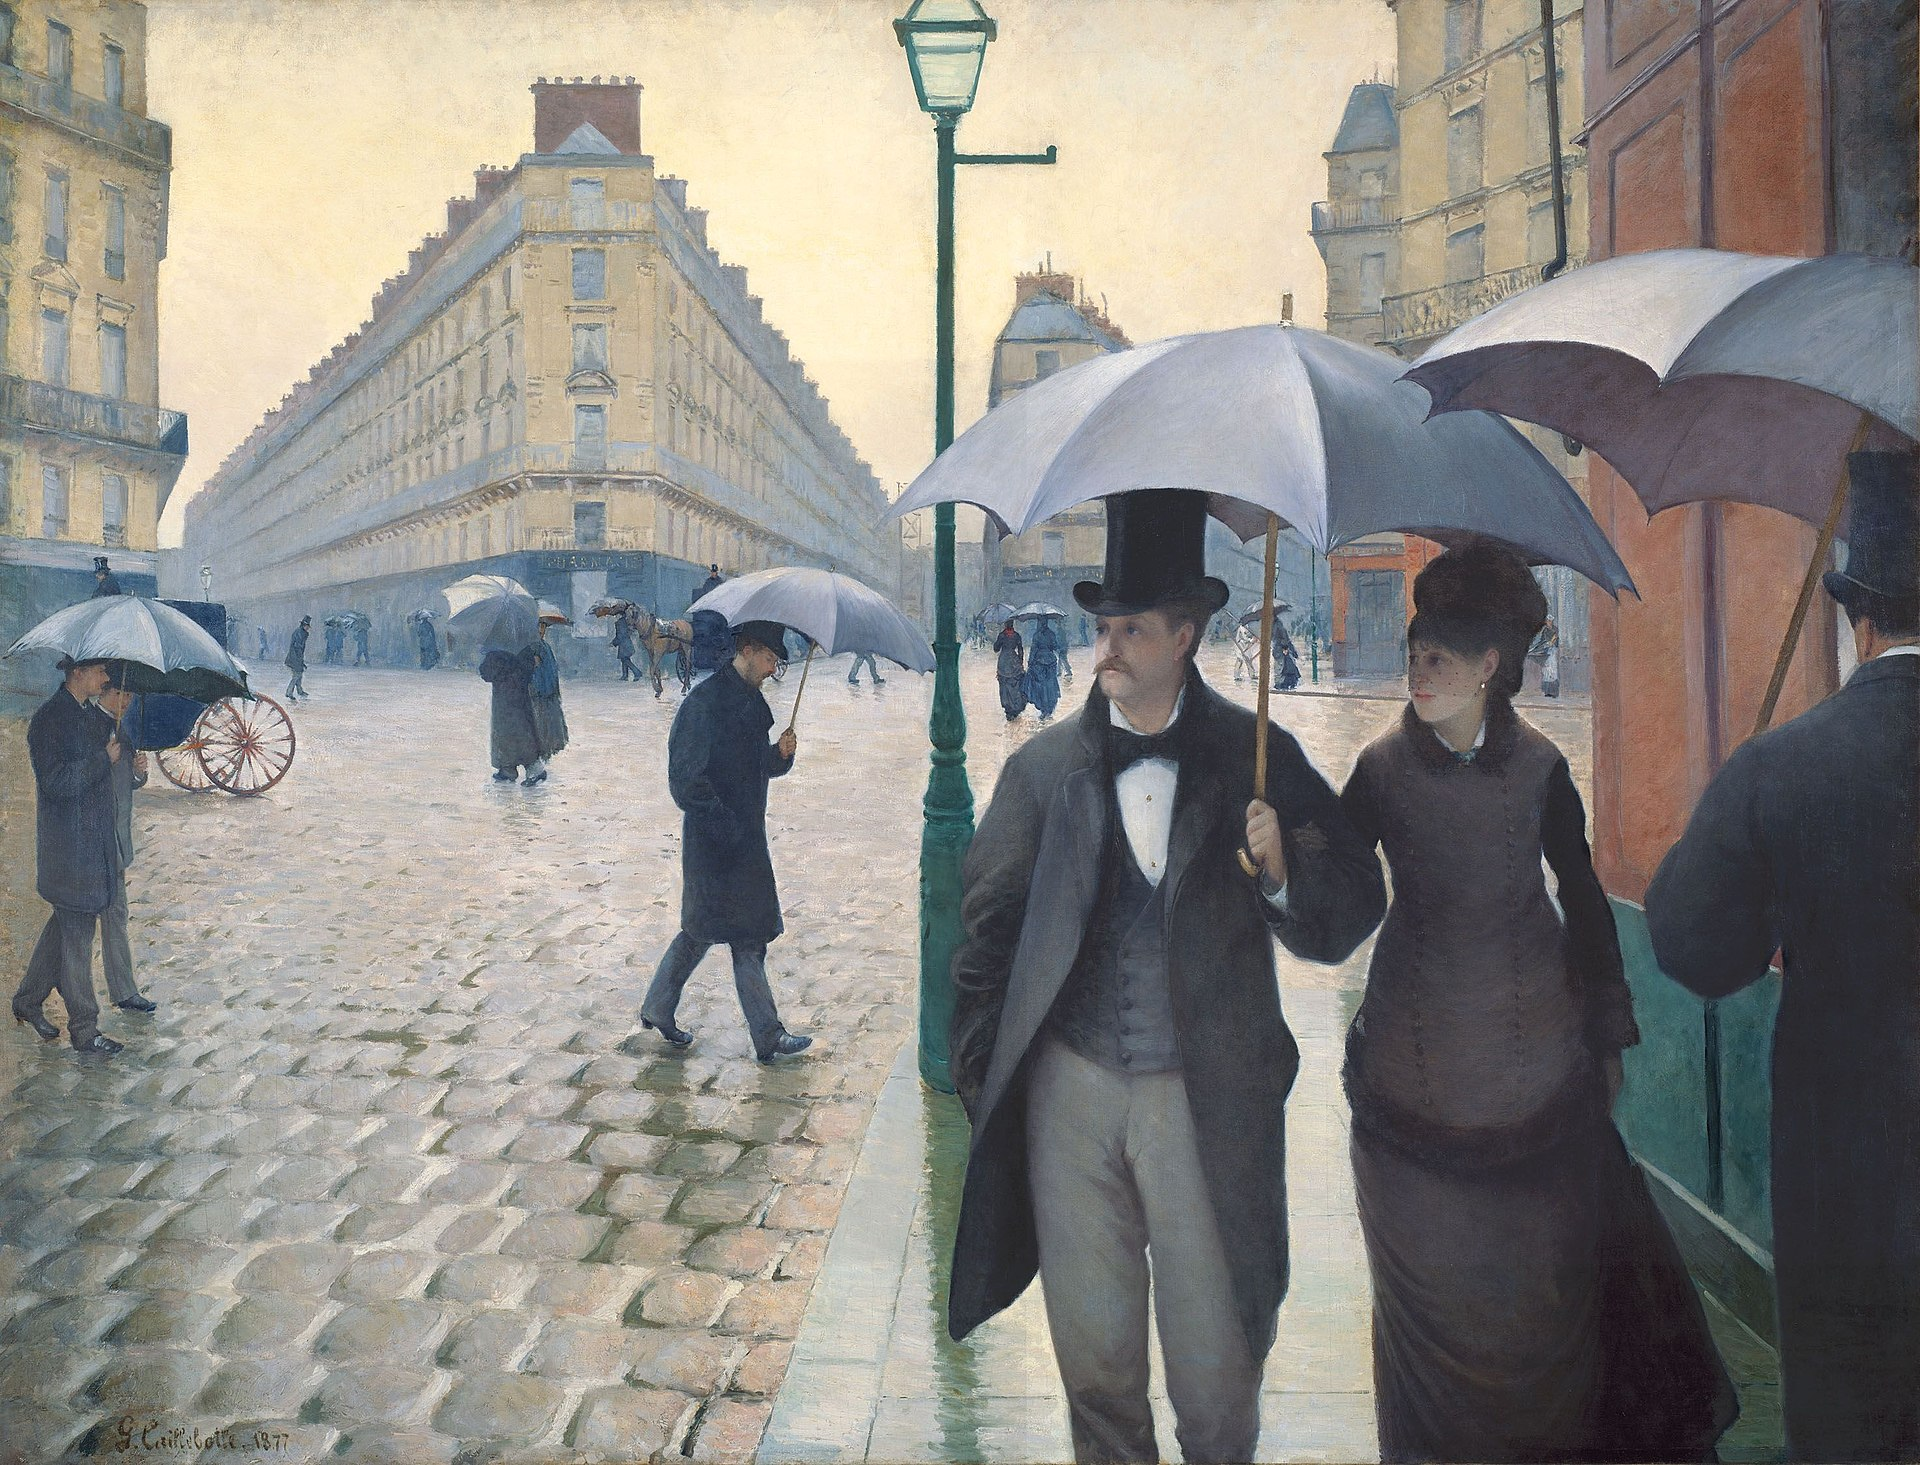
\includegraphics[width=0.6\textwidth]{img/Paris}

      \caption{Quelle: Wikipedia}
\end{figure}


\end{frame}


\begin{frame}
    \frametitle{Einleitung}
\framesubtitle{}
   \begin{block}{Stochastik vs. Kausalität}
Korrelation $\neq$ Kausalität! Aus stochastischen Zusammenhängen (Korrelationen) lassen sich \textbf{nicht} direkt kausale Zusammenhänge ableiten. 
\end{block}

   \begin{block}{Problem: Scheinkorrelation (Confounding)}
Zwei Größen $X$, $Y$ können korreliert sein, weil eine dritte Variable $Z$ (Confounder) beide beeinflusst:
$Z \to X$ und $Z \to Y$, aber $X \not\to Y$.
\end{block}

   \begin{block}{Wie kann man doch auf Kausalität schließen?}
\begin{itemize}
\item \textbf{Randomisierte Experimente:} Man teilt Teilnehmer zufällig in Gruppen ein (z.\,B. Medikament vs. Placebo). Dadurch werden alle störenden Einflüsse herausgemittelt.
\item \textbf{Gezielte Eingriffe (Interventionen):} Man verändert aktiv eine Variable und beobachtet, ob sich die andere ändert.
\end{itemize}
\end{block}

\end{frame}



\begin{frame}
    \frametitle{Einleitung}
\framesubtitle{}
\begin{block}{}
Gibt es überhaupt Zufall? 
\end{block}

\begin{figure}[htp]
      \centering
    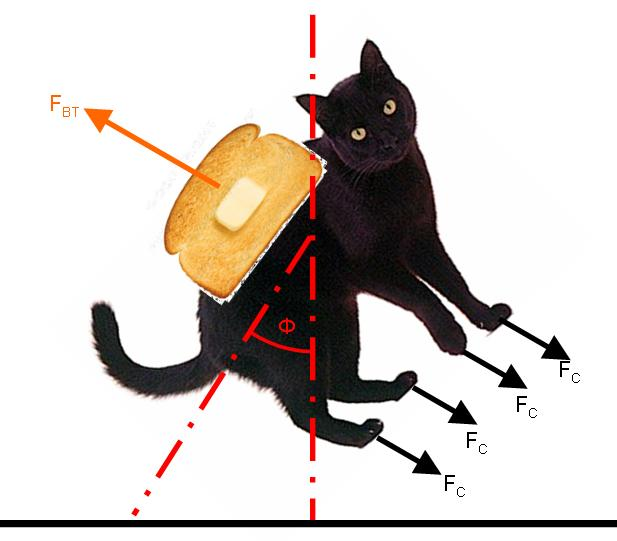
\includegraphics[width=0.2\textwidth]{img/katze-toast}

      \caption{Quelle: https://www.laurentinews.de/wp-content/uploads/2014/03/katze-toast1.jpg}
\end{figure}

    \begin{block}{}
Zufall hängt von der betrachteten Skala ab. \\
Physik $\Rightarrow$ Skalen können nicht beliebig klein werden.
\end{block}
    \begin{block}{}
\href{https://de.wikipedia.org/wiki/Brownsche_Bewegung
}{Wikipedia://Brownsche Molekularbewegung.
}
\end{block}

\end{frame}



\begin{frame}
    \frametitle{Einleitung}
\framesubtitle{}

\begin{block}{Motivation}
Maschinelles Lernen. Maschinelle Vorhersage. Informationstheorie. Prozesstheorie. Optimierungstheorie. Mustererkennung. Komplexitätstheorie, bildgebende Verfahren, Physik.
\end{block}

\begin{block}{Motivation}

Wie programmiere und trainiere ich einen "intelligenten" Spam-Filter?
Wie bewertet Google Webseiten?
Warum wird das Rauschen von Sensoren als Normalverteilt angenommen?
Macht es Sinn auf Rot zu setzen, nachdem 100 mal Schwarz im Roulette fiel?
Kann man Information quantifizieren?
Wie kann man mit einer Münze Integrale lösen und was hat das mit Hollywood zu tun? 
Ab wie vielen richtig beantworteten Ja-Nein-Fragen ist der  von meinem Kommilitonen gebaute Roboter wirklich intelligent und  hat nicht nur zufällig die richige Antwort gewählt?
\end{block}

 \end{frame}

\begin{frame}
    \frametitle{Einleitung}
\framesubtitle{}

\begin{block}{Literatur}
\begin{itemize}
\item Achim Klenke; Wahrscheinlichkeitstheorie; Springer
\item \href{https://lean-lang.org/learn/}{Learn Lean 4} (für formale Beweise)
\item Stochastik für Informatiker; L. Dümbgen; Springer
\item Einführung in die Wahrscheinlichkeitstheorie und Statistik; Hans-Otto Georgii; De Gruyter Studium
\end{itemize}
\end{block}
 \end{frame}


\begin{frame}
    \frametitle{Einleitung}
\framesubtitle{}

\begin{block}{Bessere Entscheidungen durch Mathematik?!?}
Gegeben sind 3 geschlossene Türen.  Hinter einer ist der Hauptgewinn, hinter zwei eine Ziege.
Der Spieler darf  sich zuerst für eine Tür entscheiden. 
Danach öffnet der Moderator eine der  nicht gewählten Türen, hinter der nicht der Hauptgewinn ist und fragt den Spieler, oben er seine vorige Entscheidung revidieren und die andere geschlossene Tür öffnen möchte.
\end{block}

\begin{figure}[htp]
      \centering
    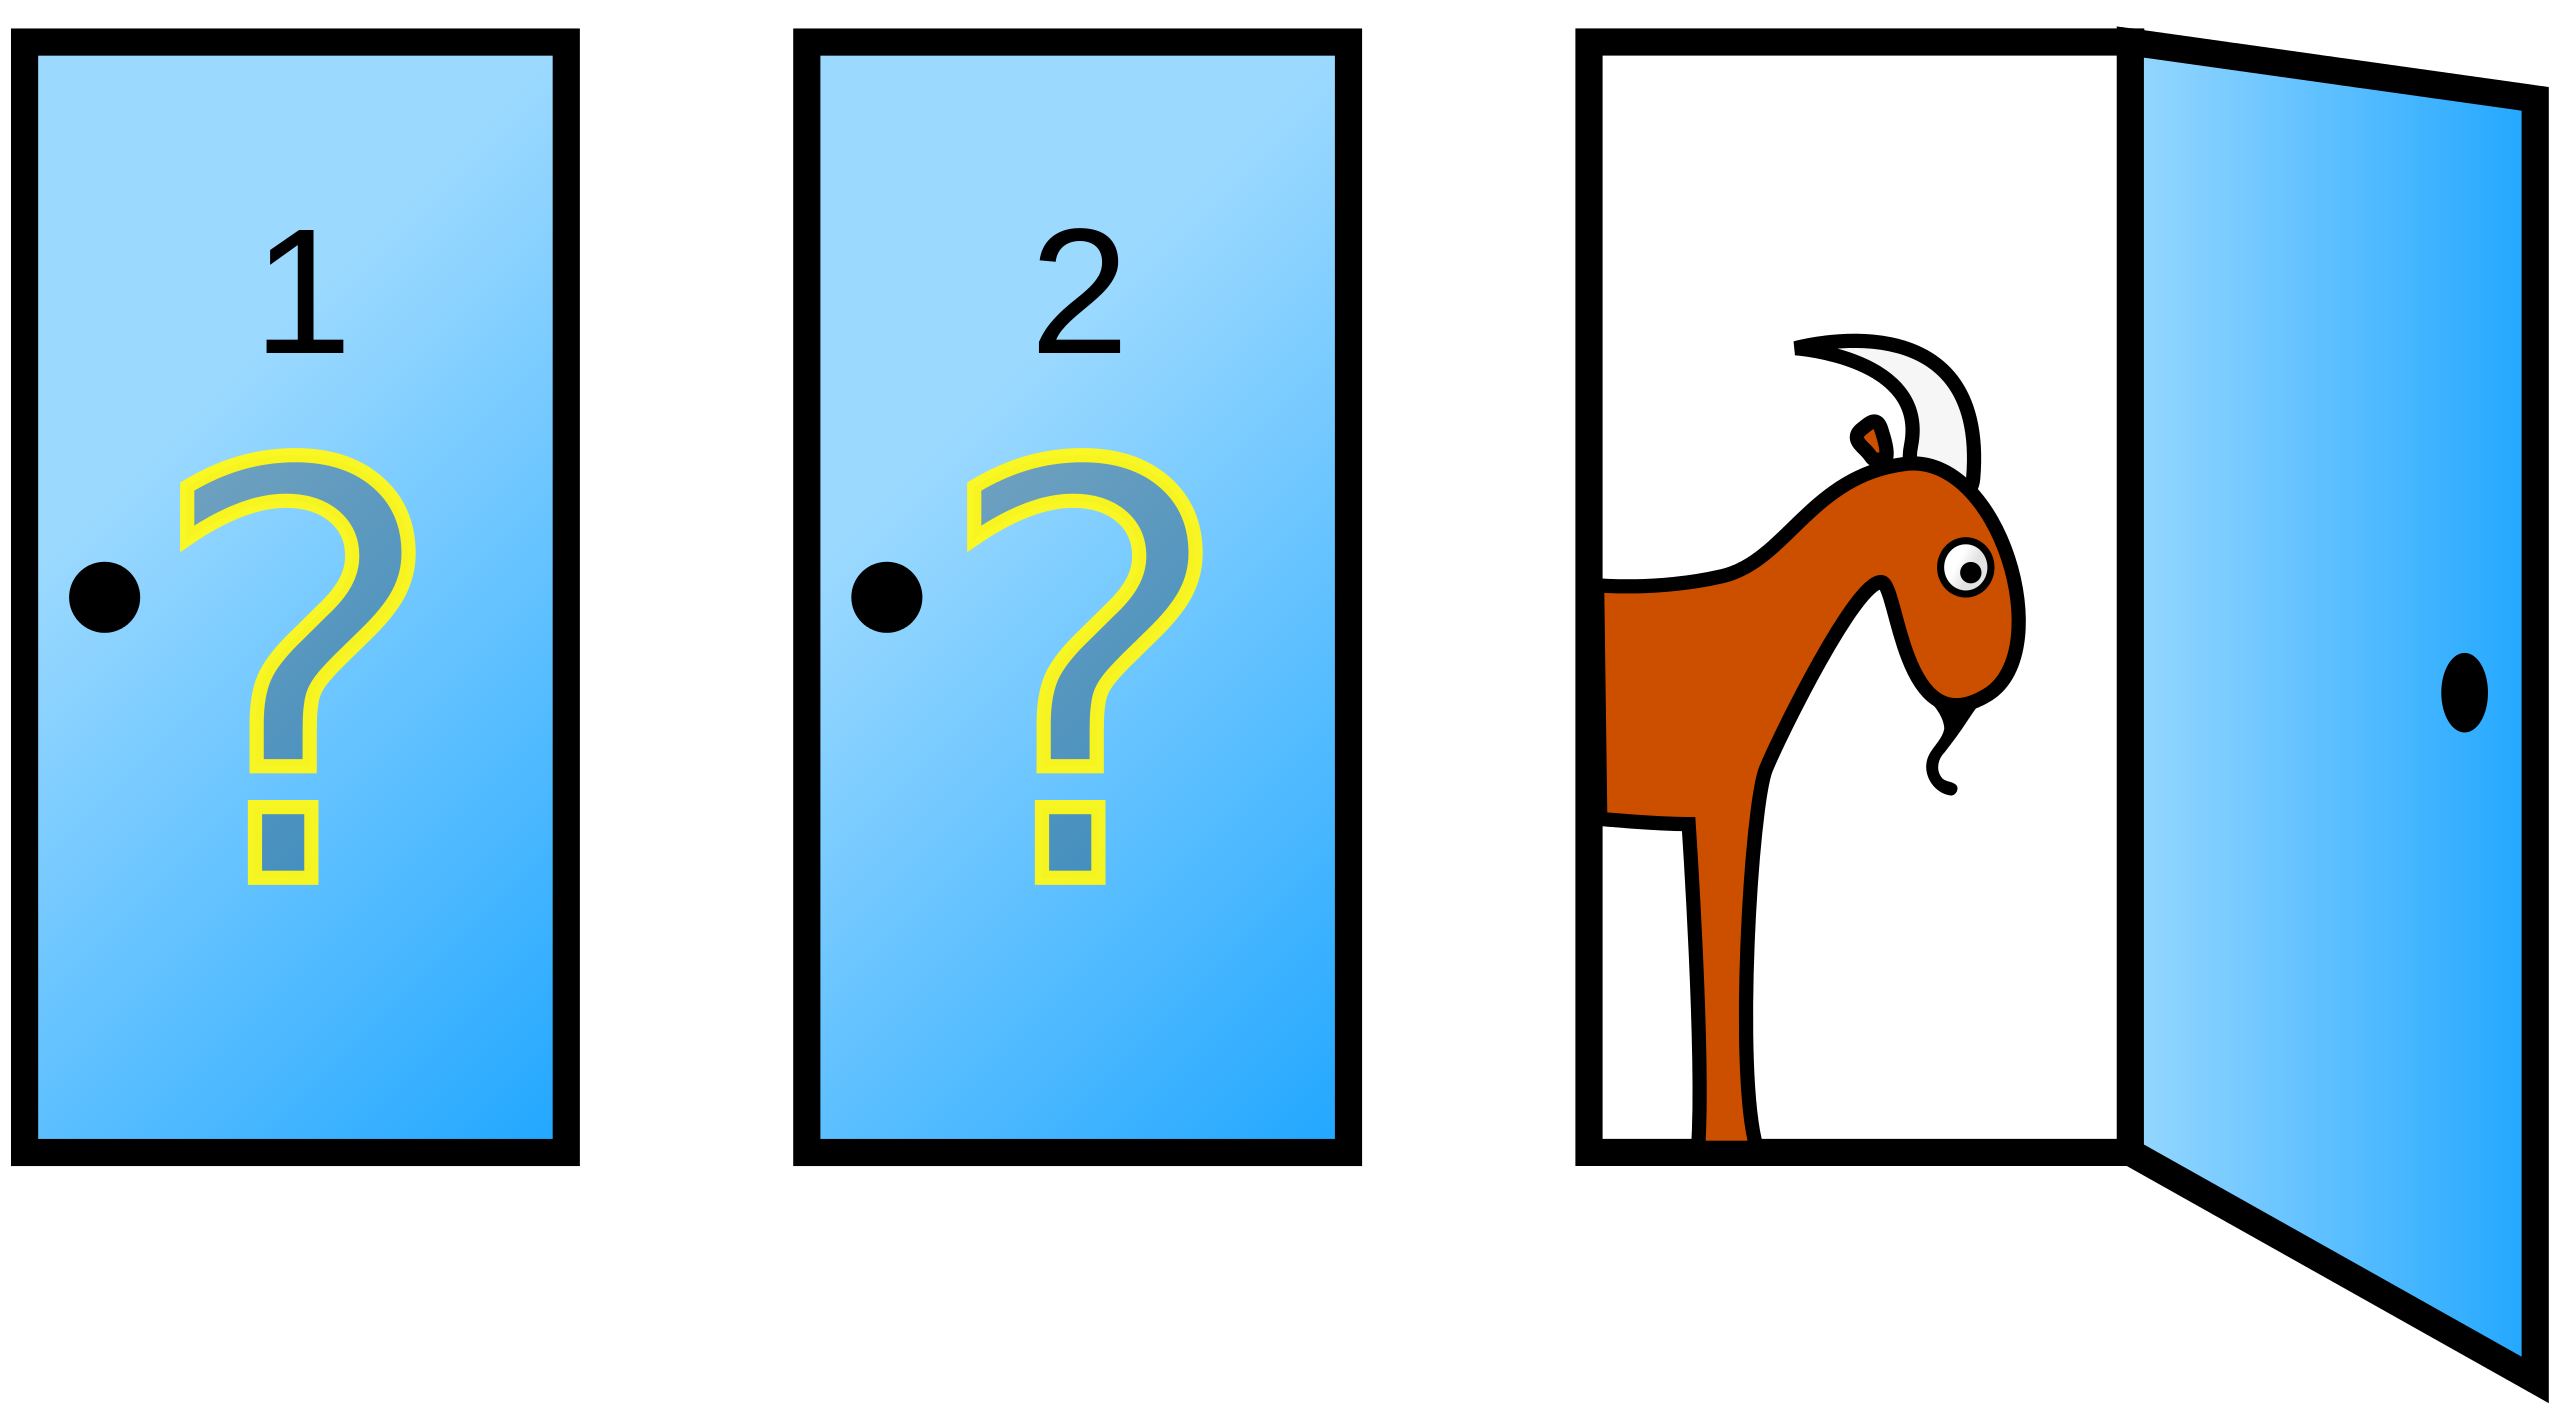
\includegraphics[width=0.45\textwidth]{img/Monty_open}

      \caption{Quelle: Wikipedia}
\end{figure}

 \end{frame}

\begin{frame}
    \frametitle{Einleitung}
\framesubtitle{}

\begin{block}{Bessere Entscheidungen durch Mathematik?!?}
Hat der Spieler eine höhere Gewinnchance, wenn er die Tür wechselt?
\end{block}

 \end{frame}

\begin{frame}
    \frametitle{Einleitung}
\framesubtitle{}

\begin{block}{Informeller Beweis}
Wechseln hat eine höhere Gewinnchance!
Ist dieser Beweis überzeugend? Geht es auch formeller?
\end{block}

\begin{figure}[htp]
      \centering
    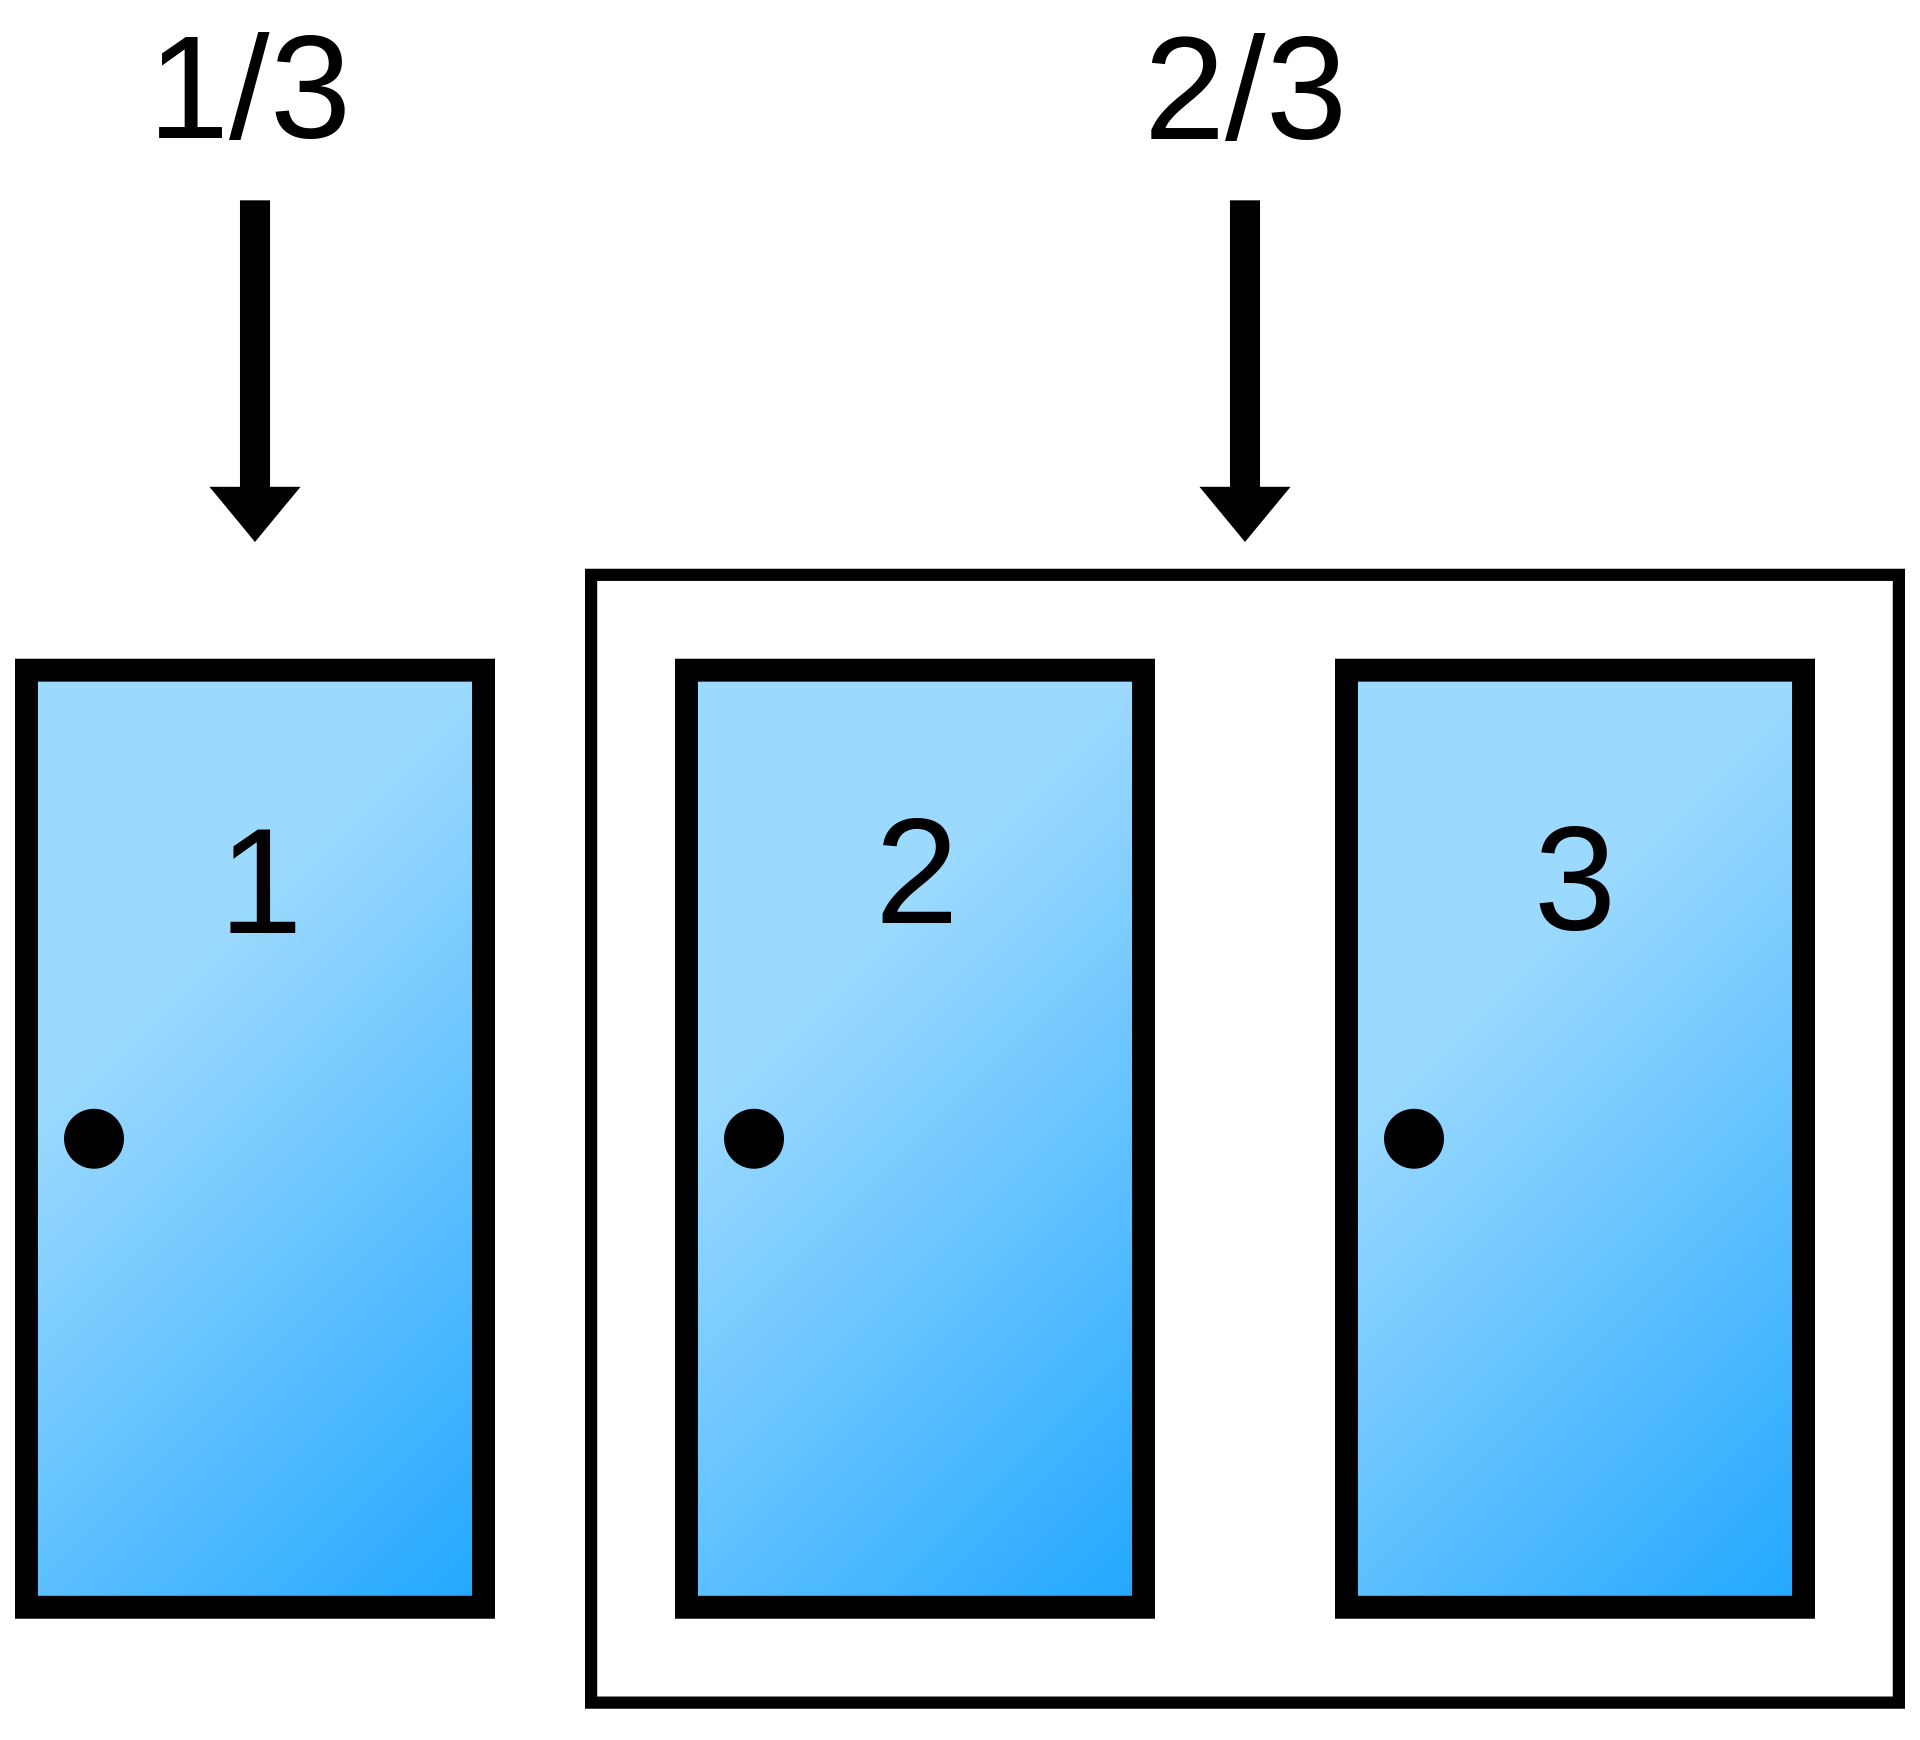
\includegraphics[width=0.45\textwidth]{img/Monty_closed_1}
    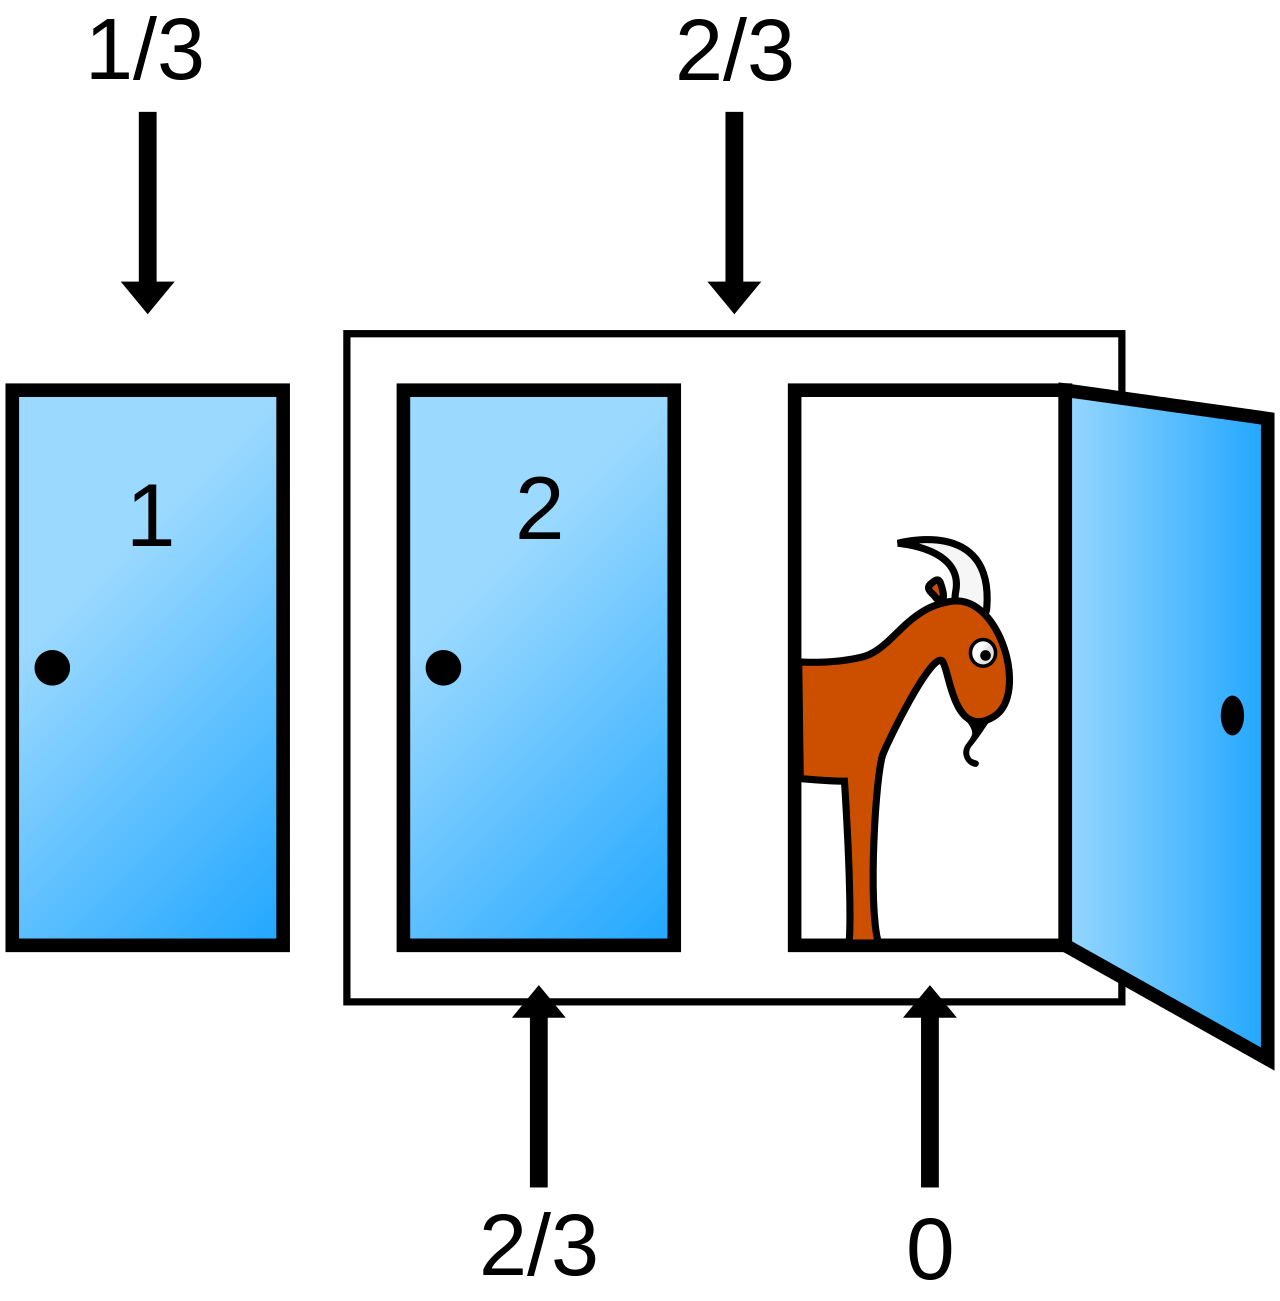
\includegraphics[width=0.45\textwidth]{img/Monty_open_1}
      \caption{Quelle: Wikipedia}
\end{figure}

 \end{frame}





\begin{frame}
    \frametitle{Einleitung}
\framesubtitle{}

\begin{block}{Was ist ein Beweis? }
Beweis des Satzes von Pythagoras der Babylonier ca. 1000 v. Chr.
\end{block}

\begin{figure}[htp]
      \centering
    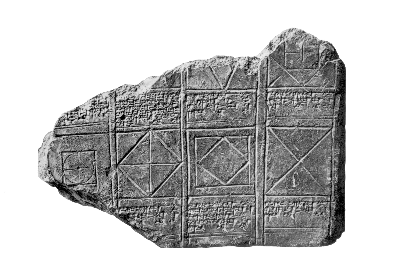
\includegraphics[width=0.6\textwidth]{img/babylon.png}

      \caption{Quelle: https://personal.math.ubc.ca/~cass/courses/m308-7b/babylon.html}
\end{figure}

 \end{frame}

\begin{frame}
    \frametitle{Einleitung}
\framesubtitle{}

\begin{block}{Was ist ein Beweis? }
Anschaulicher Beweis
\end{block}

\begin{figure}[htp]
      \centering
    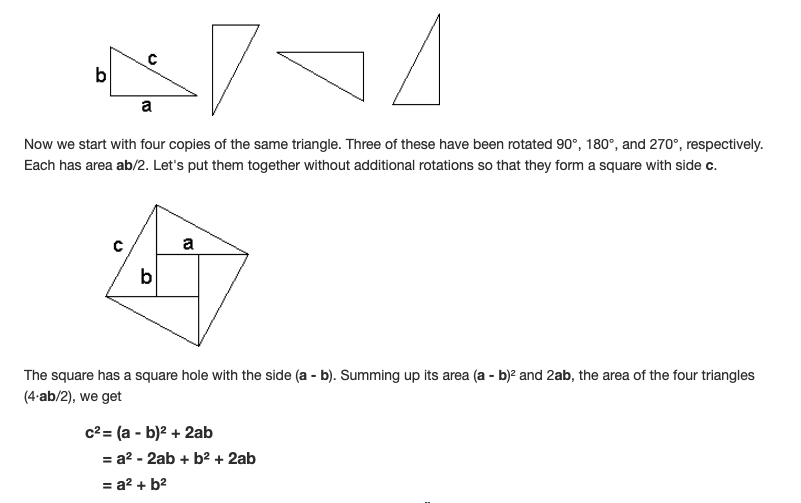
\includegraphics[width=0.8\textwidth]{img/pythagoras.png}

      \caption{Quelle: https://www.cut-the-knot.org/pythagoras/}
\end{figure}

 \end{frame}



\begin{frame}[fragile]
    \frametitle{Einleitung}
\framesubtitle{}

\begin{block}{Was ist ein Beweis? }
\href{https://github.com/leanprover-community/mathlib4/blob/9f0aee2e9bfe008c35fa9672d28e6dd4411d2971/Mathlib/Geometry/Euclidean/Angle/Unoriented/RightAngle.lean#L44-L48}{Computer überprüfbarer Beweis}:
\begin{verbatim}
/-- Pythagorean theorem, if-and-only-if
    vector angle form. -/
theorem ...iff_angle_eq_pi_div_two
  (x y : V) :
    ||x + y|| * ||x + y|| = ||x|| * ||x||
      + ||y|| * ||y||
    <-> angle x y = pi / 2 := by
  rw [...iff_real_inner_eq_zero]
  exact inner_eq_zero_iff_angle_eq_pi_div_two
    x y
\end{verbatim}
\end{block}
 \end{frame}

\begin{frame}{Drei formale Systeme im Vergleich}
\begin{block}{Mengenlehre (z.\,B. ZFC)}
{\scriptsize
\textbf{Grundobjekte:} Mengen;
\textbf{Syntax:} Formeln der Prädikatenlogik mit $\in$;
\textbf{Urteile:} $x \in A$, $A = B$;
\textbf{Axiome:} Extensionalität, Paarmenge, Vereinigung, Potenzmenge, Separation, Ersetzung, Unendlichkeit;
\textbf{Regeln:} Modus Ponens, Generalisierung, Gleichheitsregeln;
\textbf{Semantik:} Modelle der Mengenlehre}
\end{block}
\begin{block}{Kategorientheorie}
{\scriptsize
\textbf{Grundobjekte:} Objekte, Morphismen;
\textbf{Syntax:} Pfeile, Komposition, Identitäten;
\textbf{Urteile:} $f : A \to B$, $g \circ f = h$;
\textbf{Axiome:} Assoziativität, Identitätsgesetze; Produkte, Exponentialobjekte, Topoi, \ldots;
\textbf{Regeln:} Komposition, Funktorialität, universelle Eigenschaften;
\textbf{Semantik:} konkrete Kategorien als Modelle}
\end{block}
\begin{block}{Dependent Type Theory}
{\scriptsize
\textbf{Grundobjekte:} Typen, Terme, Kontexte;
\textbf{Syntax:} $A\ \mathrm{type}$, $a : A$, $\Pi$-, $\Sigma$-, Id-Typen;
\textbf{Urteile:} $\Gamma \vdash A\ \mathrm{type}$, $\Gamma \vdash a : A$;
\textbf{Axiome:} Universenaxiom, (Univalenzaxiom);
\textbf{Regeln:} Einführungs-, Eliminations-, Berechnungs- und Gleichheitsregeln;
\textbf{Semantik:} Kontextkategorien, Homotopie-Modelle}
\end{block}
\end{frame}




\begin{frame}
    \frametitle{Einleitung}
\framesubtitle{}

\begin{block}{Mathematik mit KI }
Anschauung  ubnd Intuition sind oft nicht formal korrekt, aber leichter verständlich. 
Formale Beweise sind präzise, aber schwer zu verstehen.
KI kann helfen, formale Beweise verständlicher zu machen oder anschauliche Beweise zu formalisieren.
Beweise in Computer-Form können von KI generiert und dann überprüft werden, um die Korrektheit zu gewährleisten.
\end{block}

\begin{block}{Beispiel}
Naive Mengenlehre führt zu Paradoxien wie dem Russellschen Paradoxon. 
Aber vieles, was man in naiver Mengenlehre beweisen kann, lässt sich mit kleinen Modifikationen auch formal in ZFC beweisen.
\end{block}
 
\begin{block}{Borsche Atommodel}
Das Borsche Atommodell  ist nicht korrekt, 
 trotzdem lässt sich vieles damit erklären, z.B Transistoren.
 \end{block}
\end{frame}



\end{document}
